\section{Introduction}

\subsection{Background}

Juneau, the capital city of Alaska, seamlessly combines 
breathtaking natural beauty with a rich cultural heritage. 
Nestled in the southeastern part of the state, this unique city 
is accessible only by air or sea, giving it an island-like allure 
despite being located on the mainland. Home to approximately 30,000 
residents, Juneau welcomes over a million tourists annually—a number 
that continues to grow each year. While tourism has significantly 
boosted the city’s economy, it has also brought challenges, such 
as receding glaciers, increasingly crowded streets, and rising 
carbon emissions. To ensure its long-term prosperity, Juneau 
must embrace a \textbf{sustainable tourism strategy} that balances growth 
with the preservation of its natural and cultural treasures, which will be
presented in the following sections.


\subsection{Restatement and Analyses of the Problem}

We need to complete the following tasks based on the given background
and our collected data.

\begin{itemize}
    \item \textbf{Task 1: Develop a model to quantify the tourism industry in Juneau and analyse the model.}
    \begin{itemize}
        \item The model is required to qualitatively and quantitatively analyze the factors that affect the tourism industry in Juneau, including the economy, society, and environment. 
        \item The model should be able to predict the number of tourists in the next few years and provide insights into the development of the tourism industry in Juneau.
        \item A sensitivity anslysis should be conducted to evaluate the robustness of the model.
    \end{itemize}
    \item \textbf{Task 2: Test the model's adaptability and migration capability in Sitka, Alaska.}
    \\Based on the model developed in Task 1, we need to adapt the model to the city of Sitka, Alaska, and test its adaptability and migration capability.
    \item \textbf{Task 3: Propose a sustainable tourism strategy for Juneau.}
    \\Based on the model developed in Task 1, we need to propose a sustainable tourism strategy for Juneau that balances economic growth with environmental and social sustainability.
\end{itemize}

It can be noted that task 1 serves as the foundation for Task 2 and Task 3, 
while Task 2 provides a practical application of the model developed in Task 1. 
Task 3 aims to address the challenges and opportunities identified in Task 1 and Task 2, 
providing a comprehensive and sustainable solution for the tourism industry in Juneau.

Questions can be asked to further clarify the problem:
How to quantify the tourism industry in Juneau? Which factors should be 
considered in the model and what methods should be used? After developing 
the model, how can we adapt it to another city? What suggestions and 
strategies can be proposed to promote the sustainable development of the
tourism industry in Juneau?

In summary, we should effectively build a model that can quantify the tourism
industry in Juneau, adapt the model to another city, and propose a sustainable
tourism strategy for Juneau.


\subsection{Overview of Our Work}

On the basis of the above analyses we carried out out work and the 
working framework is shown below.

\begin{figure}[H]
    \centering
    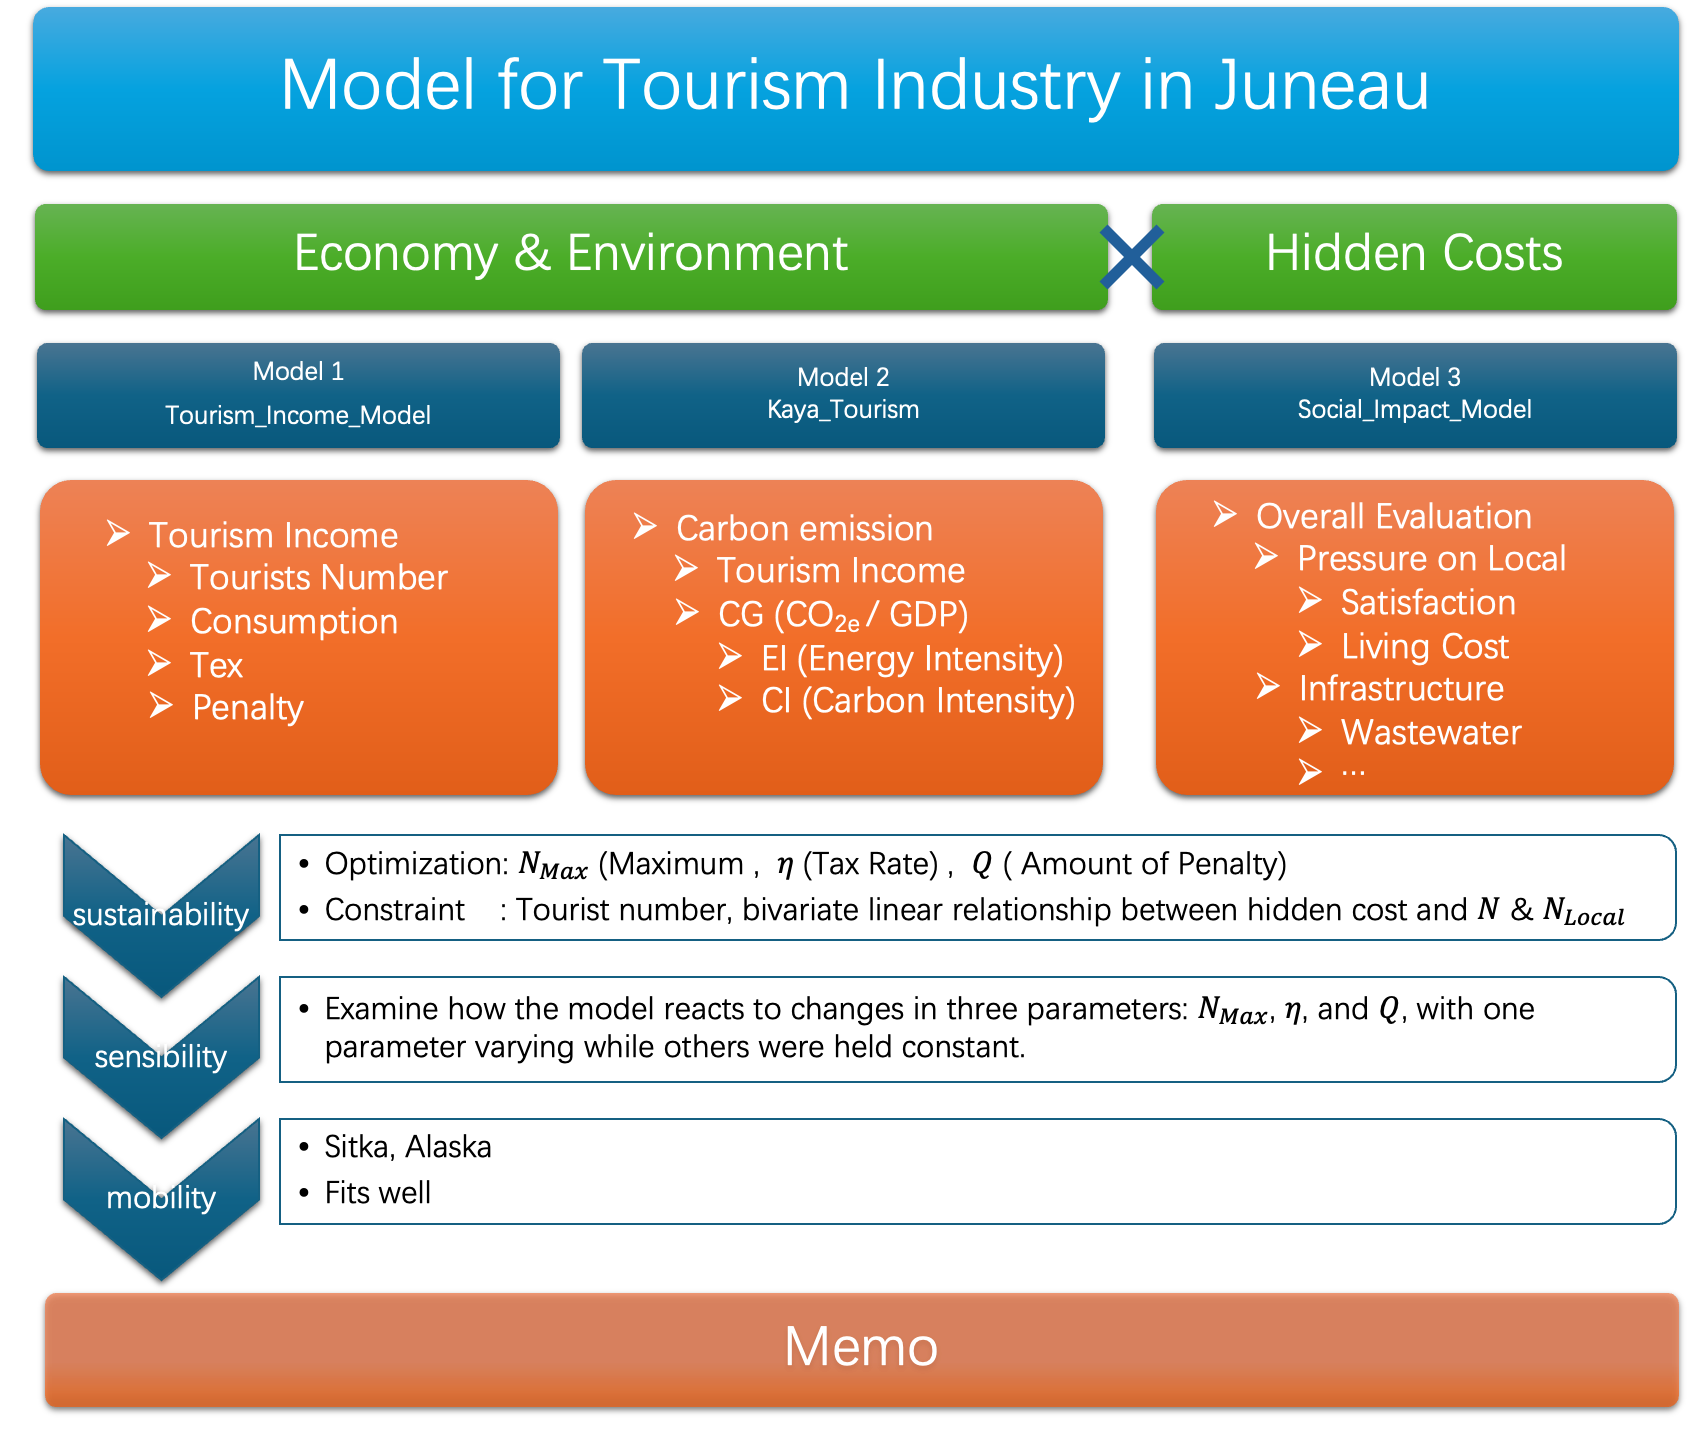
\includegraphics[width=1\textwidth]{FrameWork.jpg} % 插入图片
    \caption{Our Work Overview Schematic Diagram}
\end{figure}

